\documentclass{beamer}

\usetheme{Warsaw}
\usecolortheme{seahorse}


\usepackage[french]{babel}
\usepackage[utf8]{inputenc}
\usepackage[T1]{fontenc}


\begin{document}

\title{ Algorithmes approchés}

\author{Arpad Rimmel}
\institute{SUPELEC}

\AtBeginSection[]
{
    \begin{frame}
        \frametitle{Table des matières}
        \tableofcontents[currentsection]
    \end{frame}
}


\begin{frame}
    \titlepage
\end{frame}

\begin{frame}
    \frametitle{Table des matières}
    \tableofcontents[]
\end{frame}


\section*{Introduction}


\begin{frame}
    \frametitle{Exemple de problème}
    \begin{center}
        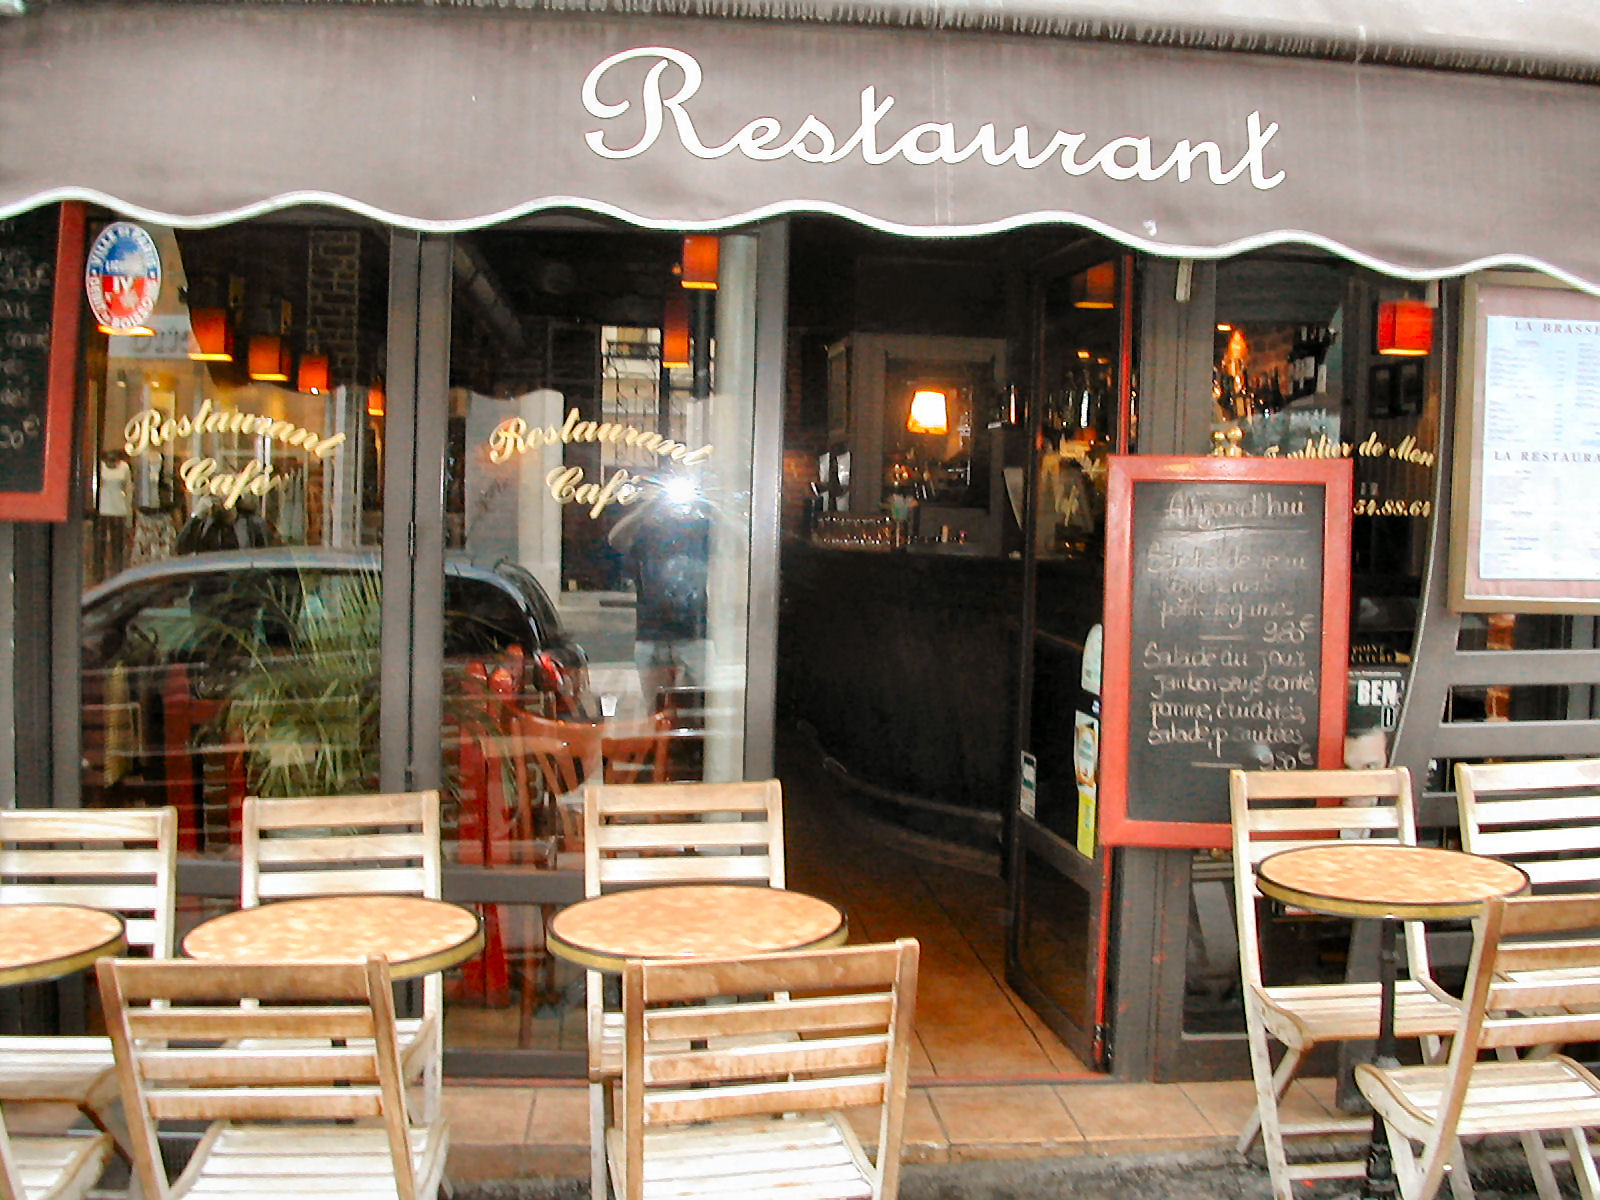
\includegraphics[scale=0.05]{restau.jpg}
    \end{center}
    Solutions?:
    \begin{itemize}
        \item Tester chaque restaurant 10 fois?
        \item Tester chaque restaurant 4 fois puis les 3 meilleurs 20 fois?
        \item Tester chaque restaurant 1 fois puis les 3 meilleurs 30 fois?
    \end{itemize}
\end{frame}


\section{Monte Carlo Tree Seach}



\section{Carrés latins}




\section*{Conclusion}

\begin{frame}
    \frametitle{conclusion}
    \begin{itemize}
        \item Le problème de bandit classique a beaucoup été étudié et de nombreux algorithmes ont été proposés qui possèdent de bonnes performances en théorie et en pratique.
        \item En fonction de l'application, une variante du bandit doit être utilisée. 
        \item Beaucoup de variantes du bandit n'ont pas ou peu été étudiées.
        \item L'utilisation de bandits pour explorer des arbres donne de bons résultats en pratique mais a peu été étudié de manière théorique.
    \end{itemize}
\end{frame}



\end{document}
